\section{نرم افزار محاسبه ضریب زلزله (\lr{CFactor})}
توسط این نرم افزار کاربر میتواند ضریب زلزله را مطابق با ویرایش چهارم آیین نامه ۲۸۰۰ بدست آورد. علاوه بر این امکانات دیگری هم در این نرم افزار گنجانده شده که انشالله به مرور زمان تکمیل خواهد شد. ویژگی های کلی

\begin{itemize}
    \item اعمال ضریب زلزله در فایل ایتبز
    \item محاسبه ضریب زلزله دریفت
    \item ساخت فایل طیف طراحی
    \item کنترل دریفت
\end{itemize}

\subsection{اعمال ضرایب زلزله در فایل ایتبز}
در حال حاضر امکانات مربوط به ایتبز برای ایتبزهای ۲۰۱۸ به بعد کار میکند. برای این منظور بعد از محاسبه ضریب زلزله و زمانیکه فایل ایتبز باز است، از منوی
$ETABS \rightarrow Export to Etabs$
برای اعمال ضریب زلزله در فایل ایتبز استفاده کنید. اگر سازه در حالت تحلیل شده قرار داشته باشد، نرم افزار به طور خودکار قفل آنرا باز میکند و سپس ضرایب زلزله را در فایل ایتبز اعمال میکند.

\begin{itemize}
    \item نرم افزار به طور خودکار جهات \lr{X, Y} و همچنین زلزله های دریفت را تشخیص میدهد.
    \item گاهی اوقات در بعضی از فایلها این کار به درستی صورت نمیگیرد. اگر بعد از اعمال ضریب زلزله، نتوانستید فایل را اجرا کنید، نگران نباشید. فایل را بسته و دوباره باز کنید. هنوز به طور دقیق علت این ایراد را متوجه نشده ام، در صورت برخورد با این مشکل فایل را برای من ارسال کنید تا مشکل اینگونه فایل ها را بررسی کنم.
\end{itemize}

\subsection{محاسبه ضریب زلزله دریفت}
با توجه به زمان تناوب های تحلیلی سازه که توسط کاربر وارد میشود، نرم افزار اقدام به محاسبه ضریب زلزله دریفت مینماید. 

\subsection{ساخت فایل طیف طراحی}
فایلهای آماده زیادی برای وارد کردن طیف طراحی در نرم افزار ایتبز وجود دارد، ولی اکثر آنها تنها چند پارامتر را مدنظر قرار میدهند مثل نوع خاک و شتاب مبنای طرح، ولی با توجه به گستردگی سیستم های باربر جانبی که ضریب رفتارهای مختلفی دارند،
ساخت همه حالتهای طیف عملا غیرممکن و غیرضروری است. ولی نرم افزار ضریب زلزله یک طیف مختص به سازه انتخاب شده برای شما ایجاد میکند که دیگر نیاز به اعمال هیچ گونه ضریبی در موقع ساخت
\lr{Load Case}
دینامیکی  در نرم افزار ایتبز وجود ندارد.
کافی است که طیف ساخته شده را مطابق شکل 
\ref{pic:spec_scale}
بدون اعمال هیچ گونه ضریب در نرم افزار ایتبز وارد کنید.

\begin{figure}
    \centering
    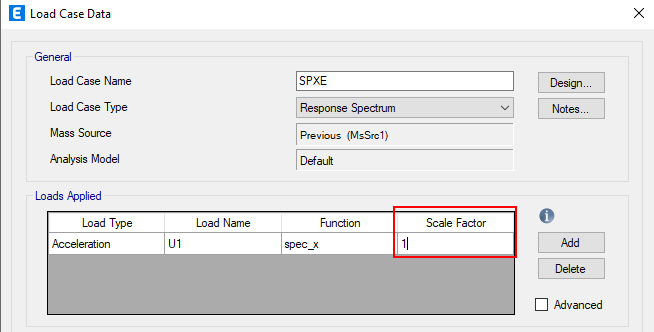
\includegraphics[scale=.7]{figures/spec_scale.png}
    \caption{نحوه ساخت حالت بار دینامیکی بدون نیاز به اعمال ضریب}
    \label{pic:spec_scale}
\end{figure}

همچنین در صورتی که سیستم های جهت 
\lr{X, Y}
متفاوت باشند نرم افزار به طور خودکار برای هر جهت یک طیف مجزا درست میکند. سپس میتوانید فایل آماده شده را مطابق شکل
\ref{pic:spec}
به نرم افزار معرفی نمایید.

\begin{figure}[H]
    \centering
    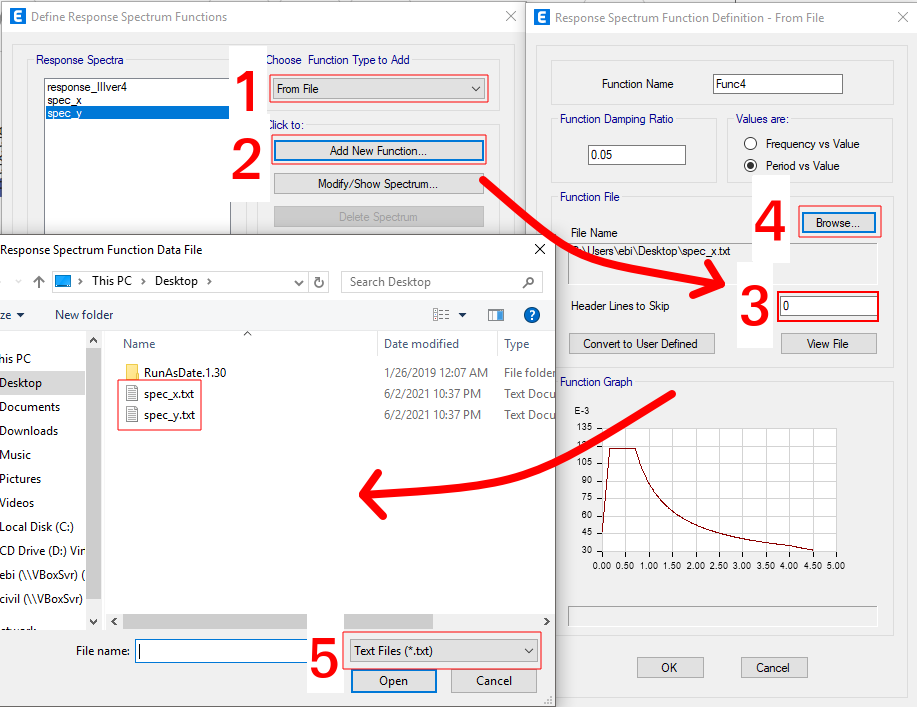
\includegraphics[scale=.7]{figures/spec}
    \caption{مراحل وارد کردن طیف به نرم افزار ایتبز}
    \label{pic:spec}
\end{figure}

\subsection{کنترل دریفت}
با استفاده از گزینه کنترل دریفت شما میتوانید با توجه به سیستم های باربر جانبی که انتخاب نموده اید و همچنین مشخص کردن تعداد طبقات سازه مقدار دریفت موجود و دریفت مجاز را برای هر راستا مشاهده کنید.
با سرچ در کادر 
\lr{Filter}
با توجه به ستون انتخاب شده در گزینه 
\lr{By Column}
، میتوانید خروجی جدول را برای مشاهده بهتر فیلتر نمایید مثلا اگر مطابق شکل
\ref{pic:drift}
گزینه ستون را
\lr{OutputCase}
انتخاب کنید، با تایپ 
\lr{dri}
فقط دریفت هایی که در نام آنها \lr{dri} باشد نمایش داده میشوند.


همچنین با کلیک روی عنوان ستونها نیز میتوانید مطابق شکل 
\ref{pic:drift_filter}
 آنها را فیلتر نمایید. فیلتر فقط روی یک ستون اعمال میشود و نمیتوان همزمان فیلتر روی چند ستون اعمال نمود، یعنی با فیلتر نمودن یک ستون، فیلتر مابقی ستونها بی اثر میشود.
 
 \begin{figure}
    \centering
    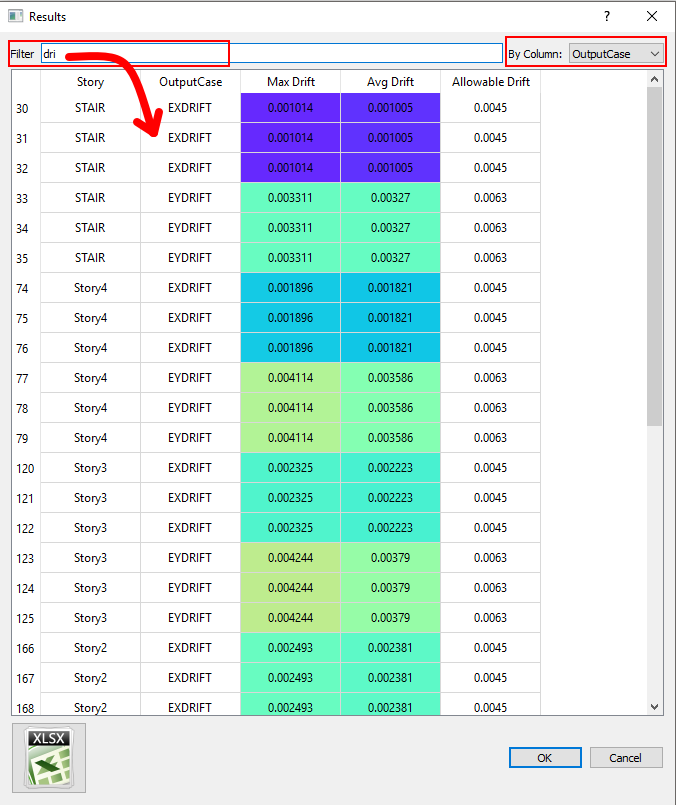
\includegraphics[scale=0.7]{figures/drift}
    \caption{فیلتر کردن خروجی جدول دریفت با انتخاب ستون مربوطه و تایپ  مقداری از محتوای ستون}
    \label{pic:drift}
\end{figure}
 
 \begin{figure}
     \centering
     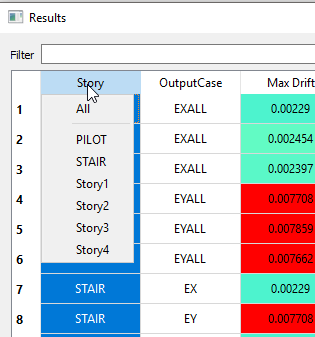
\includegraphics[scale=0.7]{figures/drift_filter}
     \caption{فیلتر کردن خروجی جدول دریفت با کلیک روی نام ستون ها}
     \label{pic:drift_filter}
 \end{figure}
 
